\documentclass[12pt]{extarticle}
\usepackage{tempora}
\usepackage[T1, T2A]{fontenc}
\usepackage[utf8]{inputenc}
\usepackage[english, ukrainian]{babel}
\usepackage{geometry}
\usepackage{graphicx}
\usepackage{multirow}
\usepackage{multicol}
\usepackage{float}
\usepackage{indentfirst}
\graphicspath{{/home/artem/Pictures}}
\geometry
{
    a4paper,
    left=30mm,
    top=15mm,
    right=20mm,
    bottom=15mm,
}

\begin{document}
\begin{titlepage}
    \begin{center}
        \textbf{\normalsize{\MakeUppercase{
            Міністерство Освіти і науки України
            Національний університет "Львівська політехніка"
        }}}

        \begin{flushright}
        \textbf{ІКНІ}\\
        Кафедра \textbf{ПЗ}
        \end{flushright}
        \vspace{15mm}

        \includegraphics[width=0.4\textwidth]{lpnu_logo.png}

        \vspace*{\fill}

        \textbf{\normalsize{\MakeUppercase{Звіт}}}
            
        До лабораторної роботи №10

        \textbf{на тему:} “Дослідження роботи протоколів ІР та ICMP.”

        \textbf{з дисципліни:} “Організація комп'ютерних мереж”
            
        \vspace*{\fill}

        \begin{flushright}

            \textbf{Лектор:}\\
            доцент кафедри ПЗ\\
            Крук О.Г.\\
            \vspace{12pt}

            \textbf{Виконав:}\\
            студент групи ПЗ-24\\
            Губик А. С.\\
            \vspace{12pt}

            \textbf{Прийняв:}\\
            доцент кафедри ПЗ\\
            Задорожний І. М.\\
        \vspace{12pt}
        \end{flushright}

        Львів -- 2023
            
            
    \end{center}
\end{titlepage}

\textbf{Тема роботи:} Дослідження роботи протоколів ІР та ICMP.
\vspace{12pt}

\textbf{Мета роботи:} Ознайомитися з принципами роботи та призначенням протоколів IP та ICMP
та за допомогою утиліт ping, tracert та аналізатора протоколів Wireshark ознайомитися зі
структурою пакетів цих протоколів
\subsection*{Індивідуальне завдання}
3 www.dlinkmea.com www.telegram.org

\subsection*{Теоретичні відомості}
Комп’ютери в мережі обмінюються даними за заздалегідь погодженим стандартом.
Такий стандарт в термінах мереж називають протоколом. Найбільш розробленими,
популярними і реалізованими у всіх операційних системах є протоколи TCP/IP.
TCP/IP (Transmission Control Protocol / Internet Protocol – Протокол управління
передачею / Протокол Internet ) – це набір протоколів, який дозволяє “безшовний” обмін
даними між комп’ютерами, незалежно від того, якого типу є ці комп’ютери, яким
підмережам вони належать і під якими операційними системами вони функціонують.
Слово “безшовний” означає, що вся реалізація передачі даних прихована від користувача
і створюється відчуття єдиної мережі. За TCP/IP передається більша частина трафіку у
крупних мережах. Саме на TCP/IP тримається Internet. Набір (комплект, стек)
протоколів означає, що в сімейство TCP/IP входять різні протоколи, основними з яких є
TCP і IP. Термін “стек”, мабуть, є найбільш правильним, оскільки TCP/IP охоплює
протоколи різних рівнів. При цьому чітко регламентована роль кожного протоколу в
цьому сімействі. Дані, якими обмінюються два комп’ютери, «курсують вгору-вниз» по
стеку TCP/IP у кожному з комп’ютерів. А саме, у комп’ютері-передавачі дані з
прикладного (найвищого) рівня (згадайте модель OSI) передаються через ряд модулів
TCP/IP, і у кожному з них “обростають” службовою інформацією визначеного формату.
Таким чином, після проходження всіх вищих рівнів дані, що підлягають передачі,
потрапляють на канальний рівень (рівень ланки даних, що забезпечується мережними
інтерфейсними платами) вже “обгорнутими” належним чином і готовими для “мандрів”
по фізичному середовищу, який є найнижчим рівнем в архітектурі мережі. На
комп’ютері-одержувачі відбувається зворотний процес – дані поетапно
“розпаковуються”, проходячи ті ж модулі TCP/IP, але в зворотному порядку, аж поки з
них не буде вичитана власне корисна інформація.
До сімейства TCP/IP належать протоколи: ARP, RARP, FTP, ICMP, IGMP, IP, TCP,
SMTP, UDP.
TCP є протоколом, що забезпечує надійну передачу потоку даних між прикладними
програмами, запущеними на різних комп’ютерах у мережі. Для цього потік даних
ділиться на TCP-сегменти на комп’ютері-відправнику, а на комп’ютері-одержувачі
відбувається повторна збірка TCP-сегментів. TCP-сегменти складаються з заголовків
TCP і даних. Надійність протоколу TCP полягає у тому, що він використовує контрольні
суми для перевірки цілісності даних і підтвердження про доставку даних.
Користувацький інтерфейс з TCP може виконувати такі команди як відкрити (OPEN) чи
закрити (CLOSE) з’єднання, відправити (SEND) чи прийняти (RECEIVE) дані або
одержати статус з’єднання (STATUS). Саме ж транспортування даних TCP “доручає”
IP-протоколу

\break
\subsection*{Хід роботи}
\paragraph{1.}
Gateway - 1.1
Phone - 1.2
Laptop - 1.3


\vspace{12pt}


\begin{figure}[H]
    \centering
    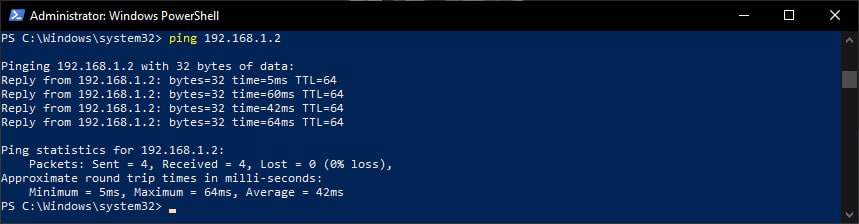
\includegraphics[width=0.90\textwidth]{ping_phone.jpg}
    \caption{}
\end{figure}


\begin{figure}[H]
    \centering
    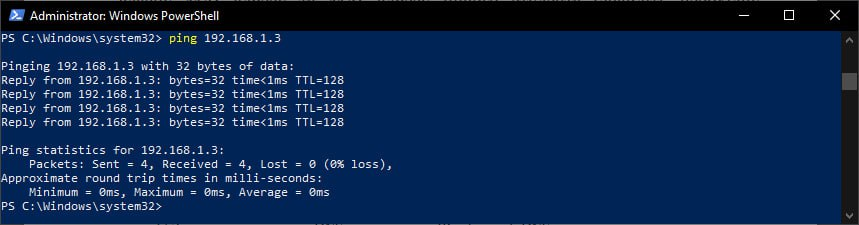
\includegraphics[width=0.90\textwidth]{ping_self.jpg}
    \caption{}
\end{figure}

\begin{figure}[H]
    \centering
    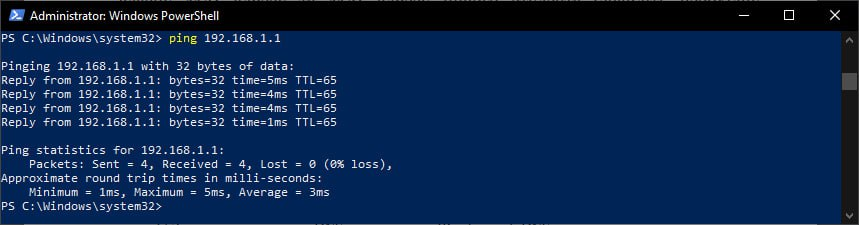
\includegraphics[width=0.90\textwidth]{ping_gateway.jpg}
    \caption{}
\end{figure}

\begin{figure}[H]
    \centering
    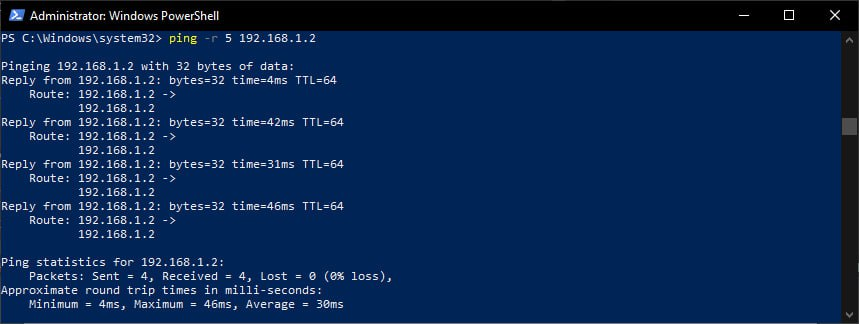
\includegraphics[width=0.90\textwidth]{ping-r.jpg}
    \caption{}
\end{figure}

\begin{figure}[H]
    \centering
    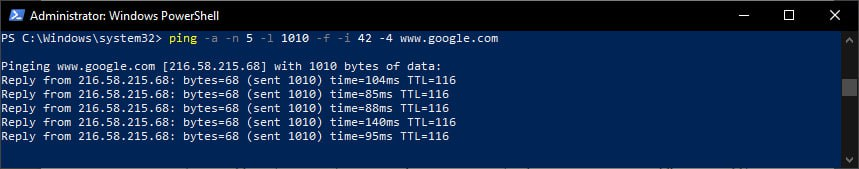
\includegraphics[width=0.90\textwidth]{ping_params.jpg}
    \caption{}
\end{figure}
\begin{figure}[H]
    \centering
    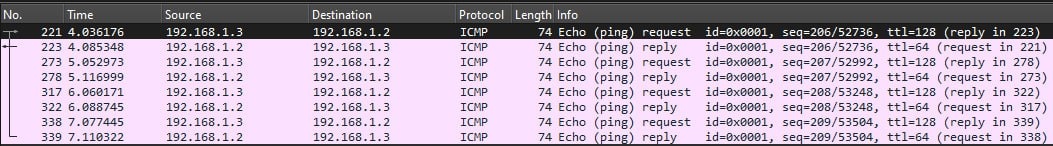
\includegraphics[width=0.90\textwidth]{icmp.jpg}
    \caption{}
\end{figure}
\begin{figure}[H]
    \centering
    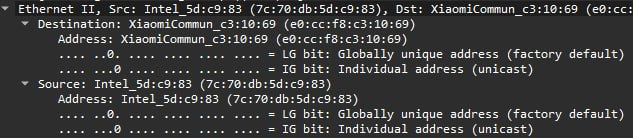
\includegraphics[width=0.90\textwidth]{icnp_phone.jpg}
    \caption{}
\end{figure}
\begin{figure}[H]
    \centering
    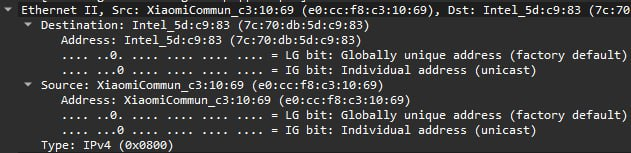
\includegraphics[width=0.90\textwidth]{icmp_laptop.jpg}
    \caption{}
\end{figure}
\begin{figure}[H]
    \centering
    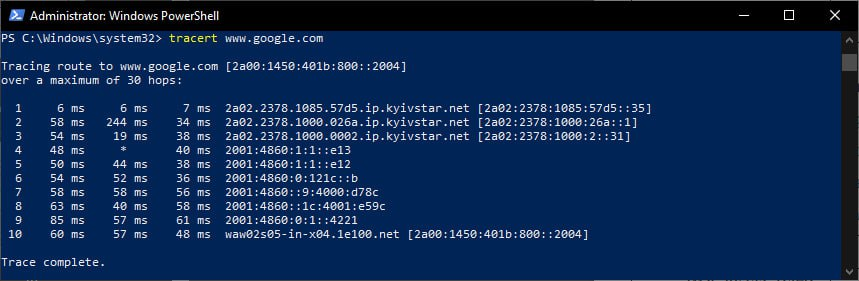
\includegraphics[width=0.90\textwidth]{tracert.jpg}
    \caption{}
\end{figure}
\begin{figure}[H]
    \centering
    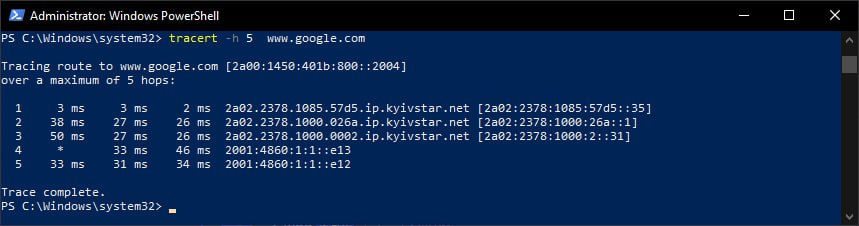
\includegraphics[width=0.90\textwidth]{tracert-d.jpg}
    \caption{}
\end{figure}
\begin{figure}[H]
    \centering
    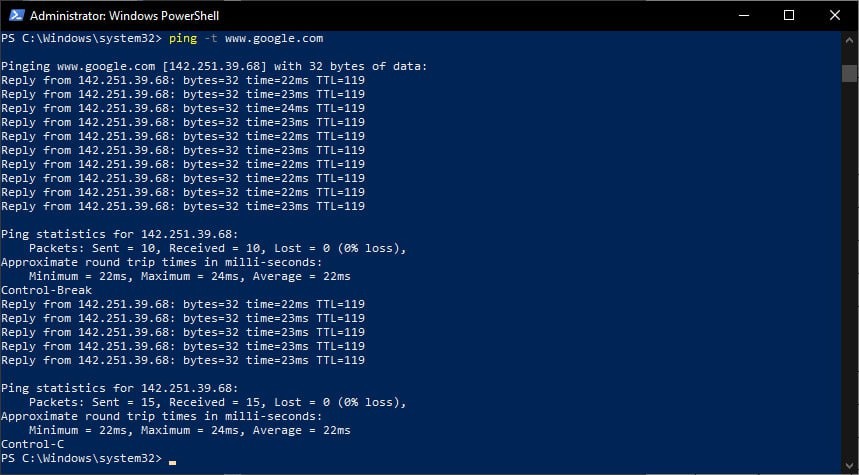
\includegraphics[width=0.90\textwidth]{tracert-t.jpg}
    \caption{}
\end{figure}
\begin{figure}[H]
    \centering
    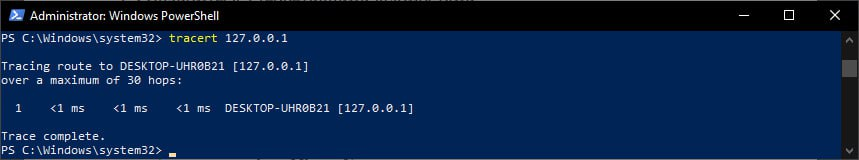
\includegraphics[width=0.90\textwidth]{tracert127.jpg}
    \caption{}
\end{figure}
\begin{figure}[H]
    \centering
    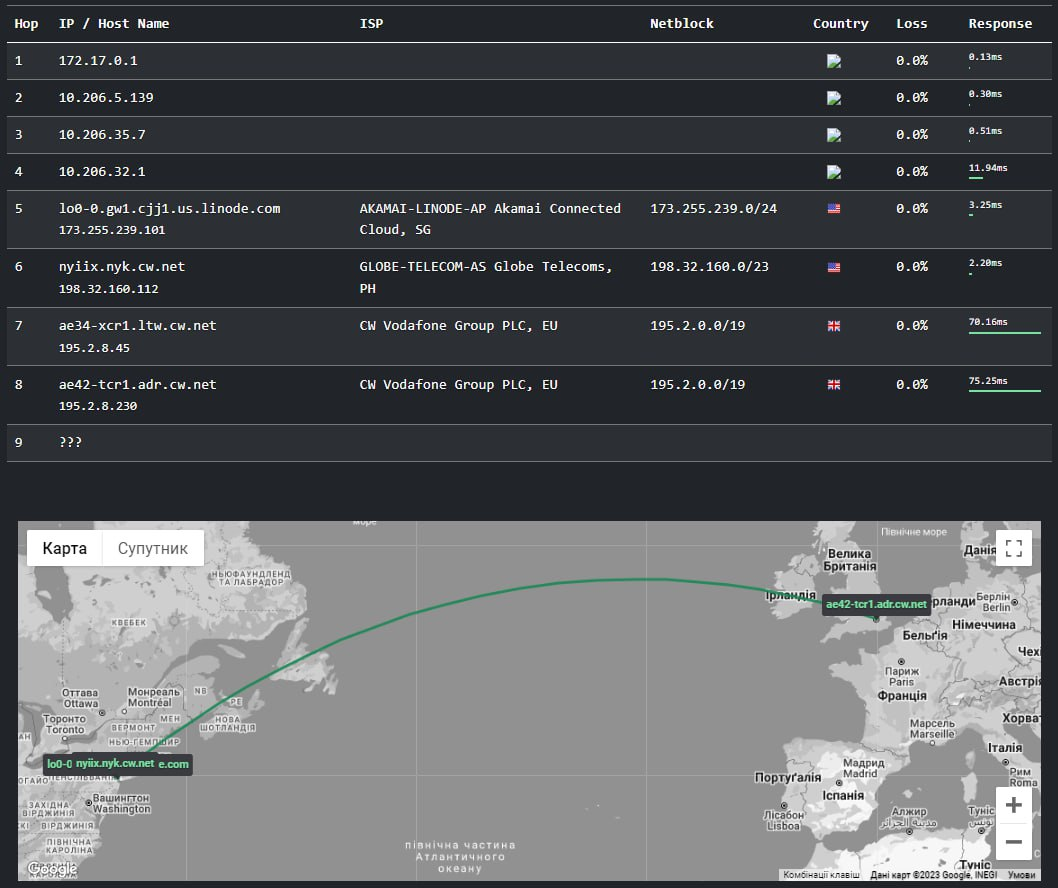
\includegraphics[width=0.90\textwidth]{tracerout.jpg}
    \caption{}
\end{figure}
\begin{figure}[H]
    \centering
    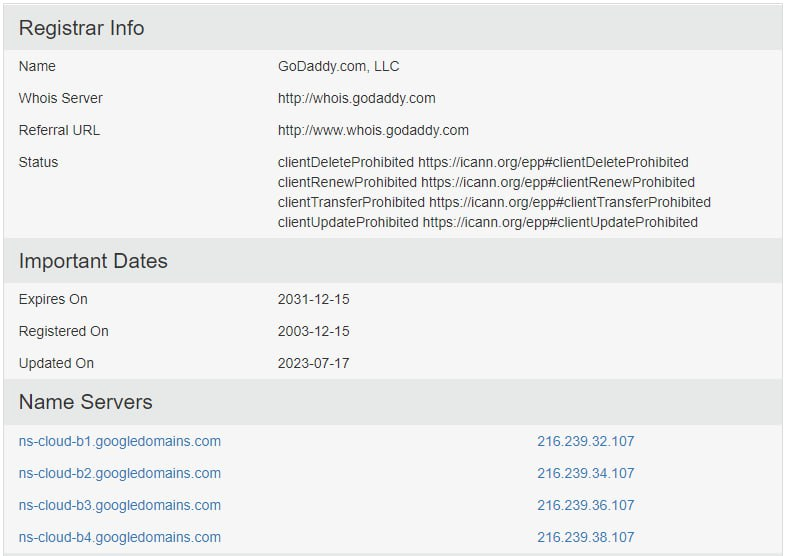
\includegraphics[width=0.90\textwidth]{whois.jpg}
    \caption{}
\end{figure}
\begin{figure}[H]
    \centering
    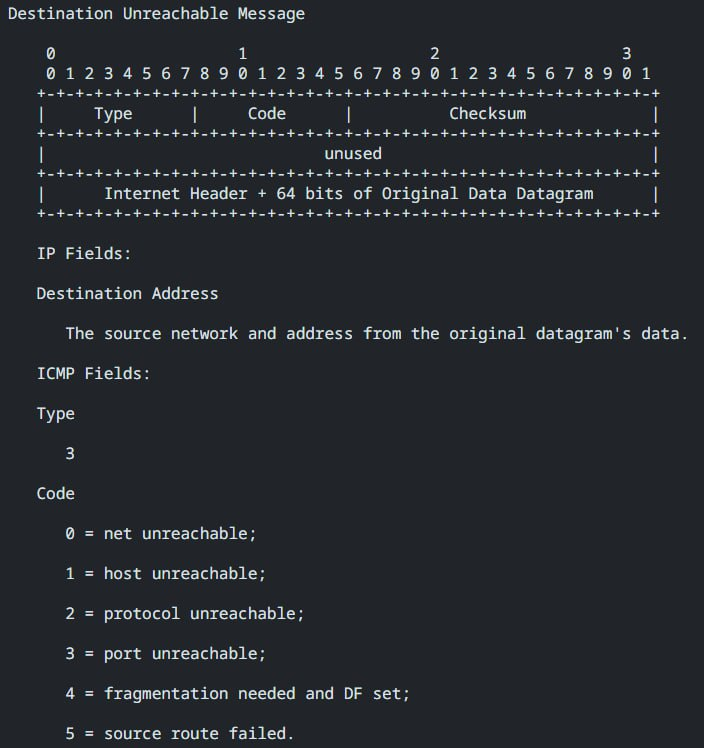
\includegraphics[width=0.90\textwidth]{rfc.jpg}
    \caption{}
\end{figure}
\vspace{12pt}

\subsection*{Висновок} 
Я навчився як користуватись командами tracert i ping з різними параметрами, 
що таке протокол ІСМР, а також як прослідкувати шлях пакета та визначити кому належить домен.
\end{document}